\subsection{Aufgabe 1: Verteilung der Zufallswerte durch \texttt{rand()}}

\texttt{rand()} liefert gleichverteilte Werte zwischen 0 und inklusive \texttt{RAND\_MAX}, d.h im Intervall \texttt{[0, RAND\_MAX]}. Untersuchen Sie, wie gut diese Gleichverteilung eingehalten wird. Dazu soll das Testprogramm zufällige Zahlen im Bereich von [1, 20] liefern. Speichern Sie die Anzahl in einem Array und stellen Sie das Resul-tat in einem GUI oder mit Hilfe von Excel dar.
Hinweis: die man-Page für die Funktion \texttt{rand()} erhalten Sie mit Hilfe des Befehls \texttt{man 3 rand}

\subsubsection{Lösung}

Das Eclipse-Projekt ist in ./Loesung/RandDist zu finden. Bei einer Umrechnung in einen bestimmten Be-reich ist wichtig, dass alle Werte, insbesondere auch der grösste und der kleinste, gleichverteilt sind. Die ein-fachste Umrechnung kann mit Hilfe des Modulooperators \% erreicht werden. Allerdings werden dann nur die niederwertigsten Bits der Zufallszahl berücksichtigt. Dies kann zu wenig zufälligen Folgen führen. Beachten Sie auch die Kommentare im Code.

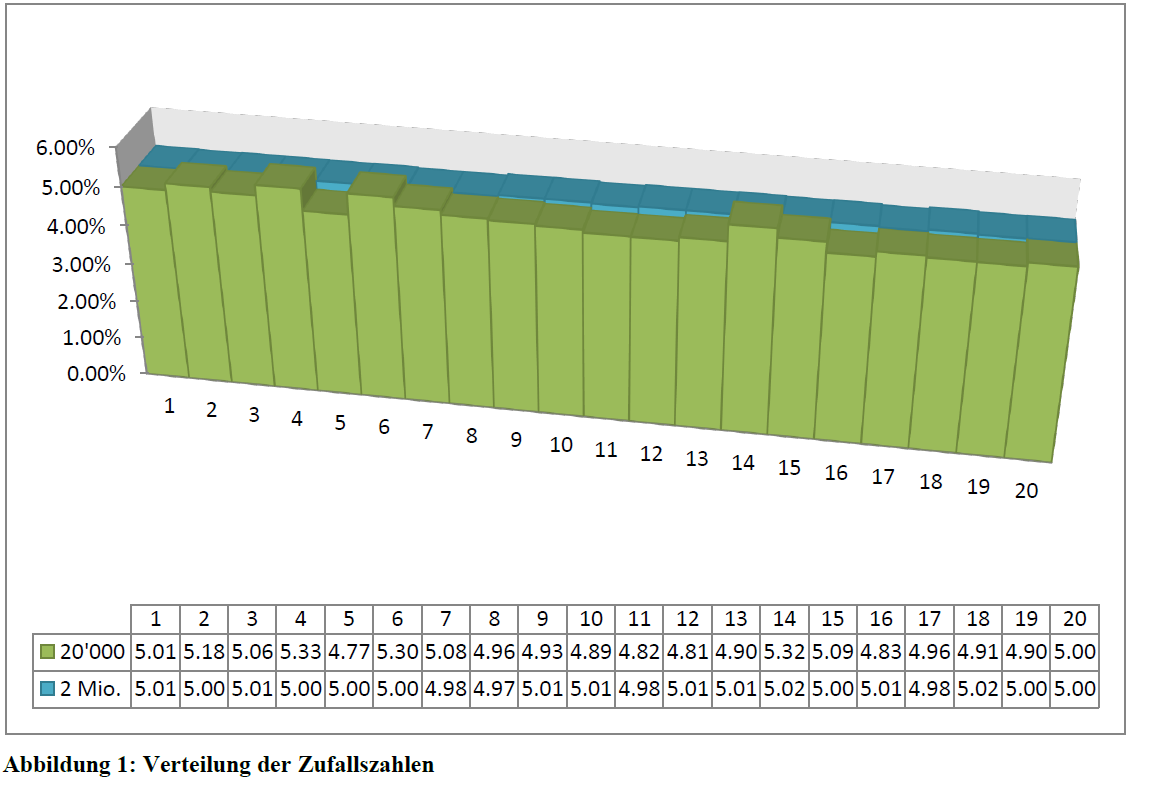
\includegraphics[width=.8\linewidth]{900-Praktika/prak04/pic.PNG}

In der folgenden Abbildung sind die Verteilungen bei 20'000, bzw. bei 2'000'000 Zufallszahlen dargestellt.

\lstinputlisting[language=C++, style=C++, multicols=2]{900-Praktika/prak04/Loesung/RandDist/src/RandDist.cpp}


\subsection{Aufgabe 2: Güte von Zufallszahlengeneratoren}
Zufallszahlen werden oft als Zahlenreihen implementiert, die mit der folgenden Formel beschrieben werden können:

\begin{equation}
  r_{i+1} = (A \cdot r_i) \% m
\end{equation}

Die Formel besteht aus einem ganzzahligen Startwert $r_0$ und mit ganzzahligen Konstanten $a$ (Multiplikator), $c $(Inkrement) und $m$ (Modulus). Diese Konstanten sind sorgfältig zu wählen, damit die Zahlen zufällig werden. So erzeugte Zahlenfolgen haben immer eine Periode $\leq$ $m$. Bei gegebenen Konstanten und Startwert $r_0$ ist die Folge eindeutig festgelegt.


Zur Beurteilung der Güte von Zufallszahlen existieren in der Statistik verschiedene Verfahren. In dieser Auf-gabe sollen Sie mit Hilfe des Computers einen graphischen Gütetest entwickeln und damit verschiedene Zu-fallszahlen-Generatoren testen. Verwenden Sie dazu Qt. Sie finden ein Qt Creator Projekt als Vorgabe.

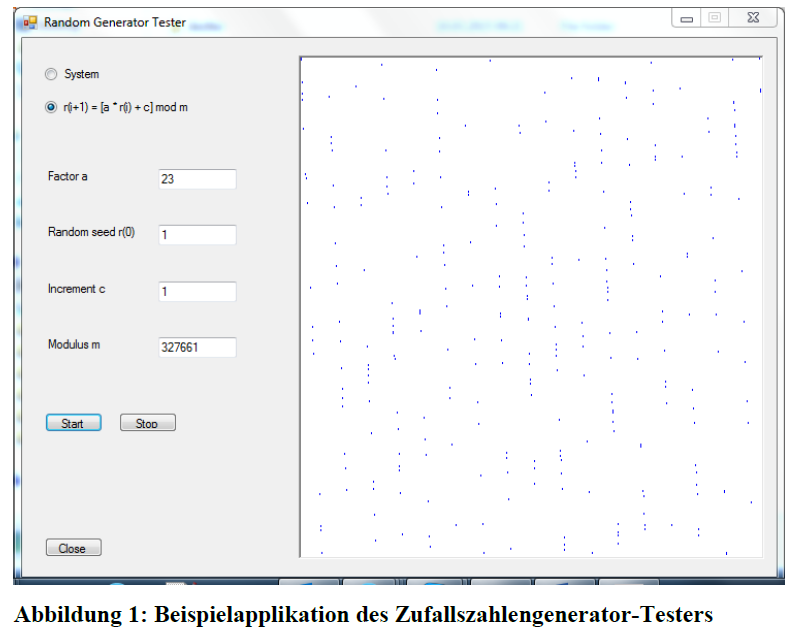
\includegraphics[width=.8\linewidth]{900-Praktika/prak04/pic2.PNG}
\begin{enumerate}
  \item Im graphischen Fenster soll ein Quadrat gezeichnet werden. Mittels zweier aufeinanderfolgender Zufalls-zahlen, die geeignet skaliert werden, wird ein Koordinatenpaar in diesem Quadrat festgelegt (1. Zufalls-zahl: x-Wert, 2. Zufallszahl: y-Wert) und an der entsprechenden Stelle ein Punkt gezeichnet. Im näch-sten Schritt wird der y-Wert zum neuen x-Wert und für den neuen y-Wert muss eine neue Zufallszahl erzeugt werden. Dieser Vorgang wird beliebig wiederholt. Durch die Beobachtung der graphischen Anordneratoren zeigen im allgemeinen ein allzu ausgeprägtes Muster. Damit das fortlaufende Zeichnen der Punkte verfolgt werden kann, wird ein Timer eingesetzt. Als Timerintervall wird 10 ms gewählt. Jedesmal wenn sich der Timer meldet, soll ein Punkt gezeichnet werden. In Ihrem Programm sollen die Werte $r_0$, $a$, $c$ und $m$ eingegeben werden können. Auf dem Skriptserver finden Sie als Muster eine vollständige ausführbare Anwendung (siehe Abbildung 1).
  \item Testen Sie z.B. die folgenden Zufallszahlengeneratoren:

  \begin{center}
           \begin{tabular}{c c c c}
           % \multicolumn{4}{ c }{\large{\textbf{Used FPGA's}}} \\
           % \multicolumn{4}{c}{} \\
           \hline
           \hline
           \textbf{$a$} &  \textbf{$r_0$} & \textbf{$c$} & \textbf{$m$} \\
           \hline

            2 & 0 & 1 & 28  \\
            8 & 0 & 1 & 7  \\
            125 & 0 & 0 & 8192  \\
            21 & 1 & 3 & 64  \\
            25 & 1 & 1 & 64  \\
            3 & 1 & 1 & 32766  \\
            130 & 1 & 1 & 32766  \\
            1331 & 1 & 1 & 327661  \\
            1103515245 & 1 & 12345 & 32768  \\

            \hline
            \hline
       \end{tabular}
   \end{center}
\item Testen Sie den Zufallszahlengenerator des Systems: rand(). Übrigens: mit Hilfe der C-Funktion srand() wird der Startwert $r_0$, der random seed, festgelegt

\end{enumerate}

\subsubsection{Lösung}

\lstinputlisting[language=C++, style=C++, multicols=2]{900-Praktika/prak04/Loesung/RandomTesterQt/main.cpp}
\noindent\makebox[\linewidth]{\rule{\paperwidth}{0.4pt}}
\lstinputlisting[language=C++, style=C++, multicols=2]{900-Praktika/prak04/Loesung/RandomTesterQt/randomtester.h}
\noindent\makebox[\linewidth]{\rule{\paperwidth}{0.4pt}}
\lstinputlisting[language=C++, style=C++, multicols=2]{900-Praktika/prak04/Loesung/RandomTesterQt/randomtester.cpp}
\noindent\makebox[\linewidth]{\rule{\paperwidth}{0.4pt}}
\lstinputlisting[language=C++, style=C++, multicols=2]{900-Praktika/prak04/Loesung/RandomTesterQt/randomviewer.h}
\noindent\makebox[\linewidth]{\rule{\paperwidth}{0.4pt}}
\lstinputlisting[language=C++, style=C++, multicols=2]{900-Praktika/prak04/Loesung/RandomTesterQt/randomviewer.cpp}

\subsection{Aufgabe 3: Nicht ideale Münze (biased coin)}
Eine ideale (faire) Münze liefert je zur Hälfte Kopf und Zahl, d.h. $p(K) = p(Z) = 0.5$. Wir nehmen nun an, die Münze sei nicht ideal, z.B.$ p(K) = 0.6, p(Z) = 0.4$.

\begin{enumerate}
  \item In ./Vorgabe/Coin/biasedCoin.cpp finden Sie die Funktion \texttt{biasedCoin()}, welche eine unfaire Mün-ze implementiert. Studieren Sie den Code und verifizieren Sie, ob die Verteilung den Erwartungen ent-spricht.
  \item Entwickeln Sie einen Algorithmus, der mit einer beliebig konstant unfairen Münze einen gleichverteilten Zufallsprozess erreichen kann. Implementieren Sie den Code, dabei müssen Sie die vorgegebene Funk-tion \texttt{biasedCoin()} nutzen und dürfen diese nicht abändern. Verifizieren Sie Ihren Algorithmus.
\end{enumerate}

Hinweis: Sie müssen die Münze zweimal hintereinander werfen.

\subsubsection{Lösung}

\begin{enumerate}
  \item Der Output in die Shell kann z.B. so aussehen: \\ 0: 5998379 (59.9838 \%) \\ 1: 4001621 (40.0162 \%)
  \item Wenn mit den gegebenen Verteilungen $p(0) = 0.6, p(1) = 0.4$ zweimal hintereinander gewürfelt wird, dann resultiert die folgende Verteilung:
  \\
  $p(00) = 0.6 \cdot 0.6 = 0.36$ \\
  $ p(11) = 0.4 \cdot 0.4 = 0.16$ \\
  $  p(01) = 0.6\cdot 0.4 = 0.24$ \\
   $p(10) = 0.4 \cdot 0.6 = 0.24$\\
Der Algorithmus sieht deshalb wie folgt aus: Es muss zweimal hintereinander gewürfelt werden. Wenn die erste Zahl 0, die zweite 1 ist, dann wird 0 zurückgegeben. Wenn die erste Zahl 1, die zweite 0 ist, dann wird 1 zurückgegeben. Wenn die beiden Zahlen gleich sind, dann müssen zwei (!) weitere Zahlen gewürfelt werden. Die letzte Zahl darf nicht be-halten und nur eine zusätzliche Münze geworfen werden. Wieso?

Weil dann mit 60 \% eine 0 kommen würde. Das würde das Resultat verfälschen.

Der Code ist unter ./Loesung/Coin/fairCoin.cpp zu finden.

Der Output kann nun so aussehen: \\ 0: 5000155 (50.0016 \%) \\ 1: 4999845 (49.9984 \%)
\end{enumerate}

\lstinputlisting[language=C++, style=C++, multicols=2]{900-Praktika/prak04/Loesung/Coin/fairCoin.cpp}
